% Options for packages loaded elsewhere
\PassOptionsToPackage{unicode}{hyperref}
\PassOptionsToPackage{hyphens}{url}
%
\documentclass[
]{book}
\usepackage{amsmath,amssymb}
\usepackage{lmodern}
\usepackage{ifxetex,ifluatex}
\ifnum 0\ifxetex 1\fi\ifluatex 1\fi=0 % if pdftex
  \usepackage[T1]{fontenc}
  \usepackage[utf8]{inputenc}
  \usepackage{textcomp} % provide euro and other symbols
\else % if luatex or xetex
  \usepackage{unicode-math}
  \defaultfontfeatures{Scale=MatchLowercase}
  \defaultfontfeatures[\rmfamily]{Ligatures=TeX,Scale=1}
\fi
% Use upquote if available, for straight quotes in verbatim environments
\IfFileExists{upquote.sty}{\usepackage{upquote}}{}
\IfFileExists{microtype.sty}{% use microtype if available
  \usepackage[]{microtype}
  \UseMicrotypeSet[protrusion]{basicmath} % disable protrusion for tt fonts
}{}
\makeatletter
\@ifundefined{KOMAClassName}{% if non-KOMA class
  \IfFileExists{parskip.sty}{%
    \usepackage{parskip}
  }{% else
    \setlength{\parindent}{0pt}
    \setlength{\parskip}{6pt plus 2pt minus 1pt}}
}{% if KOMA class
  \KOMAoptions{parskip=half}}
\makeatother
\usepackage{xcolor}
\IfFileExists{xurl.sty}{\usepackage{xurl}}{} % add URL line breaks if available
\IfFileExists{bookmark.sty}{\usepackage{bookmark}}{\usepackage{hyperref}}
\hypersetup{
  pdftitle={Biostatistics (DRAFT)},
  pdfauthor={Christopher Desjardins, Laura Le, and Ann Brearley},
  hidelinks,
  pdfcreator={LaTeX via pandoc}}
\urlstyle{same} % disable monospaced font for URLs
\usepackage{color}
\usepackage{fancyvrb}
\newcommand{\VerbBar}{|}
\newcommand{\VERB}{\Verb[commandchars=\\\{\}]}
\DefineVerbatimEnvironment{Highlighting}{Verbatim}{commandchars=\\\{\}}
% Add ',fontsize=\small' for more characters per line
\usepackage{framed}
\definecolor{shadecolor}{RGB}{248,248,248}
\newenvironment{Shaded}{\begin{snugshade}}{\end{snugshade}}
\newcommand{\AlertTok}[1]{\textcolor[rgb]{0.94,0.16,0.16}{#1}}
\newcommand{\AnnotationTok}[1]{\textcolor[rgb]{0.56,0.35,0.01}{\textbf{\textit{#1}}}}
\newcommand{\AttributeTok}[1]{\textcolor[rgb]{0.77,0.63,0.00}{#1}}
\newcommand{\BaseNTok}[1]{\textcolor[rgb]{0.00,0.00,0.81}{#1}}
\newcommand{\BuiltInTok}[1]{#1}
\newcommand{\CharTok}[1]{\textcolor[rgb]{0.31,0.60,0.02}{#1}}
\newcommand{\CommentTok}[1]{\textcolor[rgb]{0.56,0.35,0.01}{\textit{#1}}}
\newcommand{\CommentVarTok}[1]{\textcolor[rgb]{0.56,0.35,0.01}{\textbf{\textit{#1}}}}
\newcommand{\ConstantTok}[1]{\textcolor[rgb]{0.00,0.00,0.00}{#1}}
\newcommand{\ControlFlowTok}[1]{\textcolor[rgb]{0.13,0.29,0.53}{\textbf{#1}}}
\newcommand{\DataTypeTok}[1]{\textcolor[rgb]{0.13,0.29,0.53}{#1}}
\newcommand{\DecValTok}[1]{\textcolor[rgb]{0.00,0.00,0.81}{#1}}
\newcommand{\DocumentationTok}[1]{\textcolor[rgb]{0.56,0.35,0.01}{\textbf{\textit{#1}}}}
\newcommand{\ErrorTok}[1]{\textcolor[rgb]{0.64,0.00,0.00}{\textbf{#1}}}
\newcommand{\ExtensionTok}[1]{#1}
\newcommand{\FloatTok}[1]{\textcolor[rgb]{0.00,0.00,0.81}{#1}}
\newcommand{\FunctionTok}[1]{\textcolor[rgb]{0.00,0.00,0.00}{#1}}
\newcommand{\ImportTok}[1]{#1}
\newcommand{\InformationTok}[1]{\textcolor[rgb]{0.56,0.35,0.01}{\textbf{\textit{#1}}}}
\newcommand{\KeywordTok}[1]{\textcolor[rgb]{0.13,0.29,0.53}{\textbf{#1}}}
\newcommand{\NormalTok}[1]{#1}
\newcommand{\OperatorTok}[1]{\textcolor[rgb]{0.81,0.36,0.00}{\textbf{#1}}}
\newcommand{\OtherTok}[1]{\textcolor[rgb]{0.56,0.35,0.01}{#1}}
\newcommand{\PreprocessorTok}[1]{\textcolor[rgb]{0.56,0.35,0.01}{\textit{#1}}}
\newcommand{\RegionMarkerTok}[1]{#1}
\newcommand{\SpecialCharTok}[1]{\textcolor[rgb]{0.00,0.00,0.00}{#1}}
\newcommand{\SpecialStringTok}[1]{\textcolor[rgb]{0.31,0.60,0.02}{#1}}
\newcommand{\StringTok}[1]{\textcolor[rgb]{0.31,0.60,0.02}{#1}}
\newcommand{\VariableTok}[1]{\textcolor[rgb]{0.00,0.00,0.00}{#1}}
\newcommand{\VerbatimStringTok}[1]{\textcolor[rgb]{0.31,0.60,0.02}{#1}}
\newcommand{\WarningTok}[1]{\textcolor[rgb]{0.56,0.35,0.01}{\textbf{\textit{#1}}}}
\usepackage{longtable,booktabs,array}
\usepackage{calc} % for calculating minipage widths
% Correct order of tables after \paragraph or \subparagraph
\usepackage{etoolbox}
\makeatletter
\patchcmd\longtable{\par}{\if@noskipsec\mbox{}\fi\par}{}{}
\makeatother
% Allow footnotes in longtable head/foot
\IfFileExists{footnotehyper.sty}{\usepackage{footnotehyper}}{\usepackage{footnote}}
\makesavenoteenv{longtable}
\usepackage{graphicx}
\makeatletter
\def\maxwidth{\ifdim\Gin@nat@width>\linewidth\linewidth\else\Gin@nat@width\fi}
\def\maxheight{\ifdim\Gin@nat@height>\textheight\textheight\else\Gin@nat@height\fi}
\makeatother
% Scale images if necessary, so that they will not overflow the page
% margins by default, and it is still possible to overwrite the defaults
% using explicit options in \includegraphics[width, height, ...]{}
\setkeys{Gin}{width=\maxwidth,height=\maxheight,keepaspectratio}
% Set default figure placement to htbp
\makeatletter
\def\fps@figure{htbp}
\makeatother
\setlength{\emergencystretch}{3em} % prevent overfull lines
\providecommand{\tightlist}{%
  \setlength{\itemsep}{0pt}\setlength{\parskip}{0pt}}
\setcounter{secnumdepth}{5}
\usepackage{booktabs}
\ifluatex
  \usepackage{selnolig}  % disable illegal ligatures
\fi
\usepackage[]{natbib}
\bibliographystyle{apalike}

\title{Biostatistics (DRAFT)}
\author{Christopher Desjardins, Laura Le, and Ann Brearley}
\date{2021-05-24}

\begin{document}
\maketitle

{
\setcounter{tocdepth}{1}
\tableofcontents
}
\hypertarget{prerequisites}{%
\chapter{Prerequisites}\label{prerequisites}}

This is a \emph{sample} book written in \textbf{Markdown}. You can use anything that Pandoc's Markdown supports, e.g., a math equation \(a^2 + b^2 = c^2\).

The \textbf{bookdown} package can be installed from CRAN or Github:

\begin{Shaded}
\begin{Highlighting}[]
\FunctionTok{install.packages}\NormalTok{(}\StringTok{"bookdown"}\NormalTok{)}
\CommentTok{\# or the development version}
\CommentTok{\# devtools::install\_github("rstudio/bookdown")}
\end{Highlighting}
\end{Shaded}

Remember each Rmd file contains one and only one chapter, and a chapter is defined by the first-level heading \texttt{\#}.

To compile this example to PDF, you need XeLaTeX. You are recommended to install TinyTeX (which includes XeLaTeX): \url{https://yihui.org/tinytex/}.

\hypertarget{introduction-to-biostatistics}{%
\chapter{Introduction to Biostatistics}\label{introduction-to-biostatistics}}

What is \emph{Biostatistics}? How does it fit within the larger field of research? What will you learn from this course? These are the questions that will be addressed in this lecture.

Let's begin with the question ``What is statistics?''.

There are many definitions, but they all have similar themes.

For many people (maybe even you), statistics is seen as a branch of mathematics. However, John Tukey, a famous statistician in the mid-1900's, stated that ``statistics is a science, not a branch of mathematics, but uses mathematical models as essential tools.'' Just as engineering, chemistry, and economics use math as a tool but are seen as separate fields from math, so should statistics be distinguished from mathematics.

Alan Agresti and Christine Franklin have described statistics as ``the art and science of learning from data'' (this is also the title of their introductory statistics textbook). The goal of statistics is to translate data into understanding of the real world. At the heart of it all is the word data.

Examples of areas in which statistics is used include business, climate change research, manufacturing quality control, government policy, education, finance, and even sports (have you seen the movie Moneyball?).

\hypertarget{cycle-of-research}{%
\section{Cycle of Research}\label{cycle-of-research}}

Medical or public health research, like all scientific research, begins with a \emph{research question} about a population of interest. Biostatistical methods are used to help answer this research question. Let's describe this process using the Cycle of Research diagram shown here.

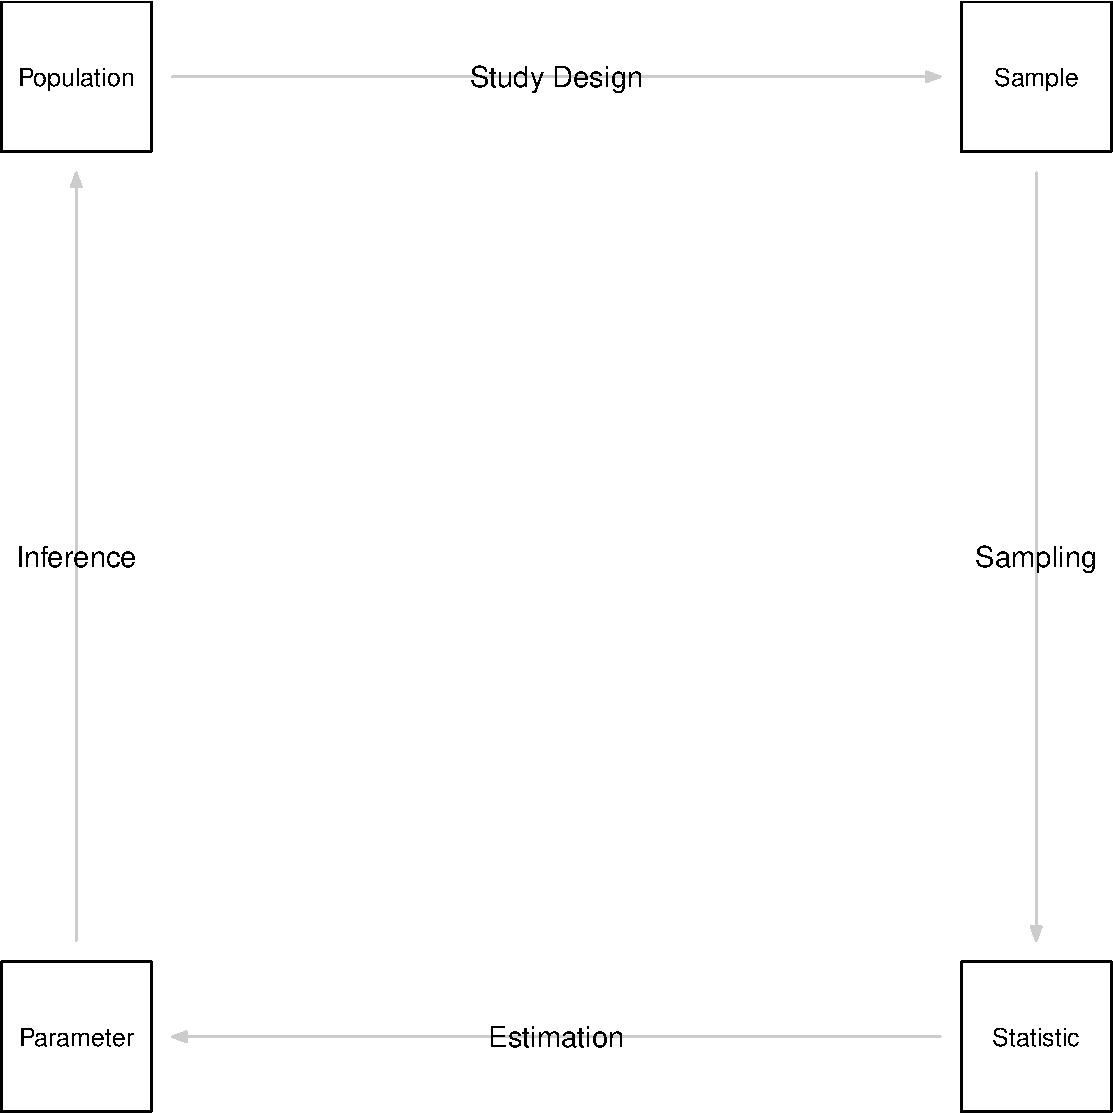
\includegraphics{biostat-book_files/figure-latex/fig.cor-1.pdf}

\hypertarget{step-1-population-to-sample}{%
\subsection{Step 1: Population to Sample}\label{step-1-population-to-sample}}

The scientific \emph{Cycle of Research} begins with a \emph{population}. A population is the complete set of individuals who share some common characteristics. The population is the group of people we are interested in learning about. The population of interest in a given study may be U.S. adult males, or it may be Finnish preschoolers, or it may be HIV-positive adults in South Africa. Perhaps we are interested, for example, in knowing how tall ten-year-old American boys are. The population in this case would be all ten-year-old boys in the U.S.

When we want to answer a specific question about a particular population, typically we obtain a sample. A \emph{sample} is a subset of the population of interest. The sample is the group of people we actually study. This is the group of people from whom data are collected. In our example, we might randomly sample 1,000 ten-year-old boys from the U.S. population to serve as our study's sample.

You may wonder, if the goal is to make some conclusions about the population, why not just collect data on the entire population? Samples are often studied instead of entire populations for several reasons.

One reason is cost. Often it would be too expensive and/or too time-consuming to collect data from an entire population of interest. For example, perhaps we are interested in the blood pressures of residents of Massachusetts. It would be much too expensive to obtain blood pressure measurements from every resident of the state, so we obtain a sample of residents instead. Take a careful look at this figure. Note that the samples have different numbers of people in them, and different mean (or average) diastolic blood pressure values. Also note that none of the mean values for the samples are the same as the mean blood pressure for the population. We will explore these concepts later.

Another reason for using a sample instead of the population is feasibility. Studying the entire population may simply not be possible. For example, it is not possible to determine the effect of a new treatment on an entire population of patients if the treatment is not yet available to the entire population.

A third reason is accuracy. Measurements from a study's sample may be more accurate than measurements from a population. More time and effort can be devoted to carrying out the measurements for the smaller number of people in the sample than is feasible for an entire population. We also can't measure everyone in the population at the same time in the same way. Measurements may change over time (as we have all seen with our weight). If we have to measure a lot of participants, we may need multiple people or instruments to do it, which can also decrease accuracy.

Finally, it may be unethical to study the entire population. If you're administering a treatment that might be harmful or withholding a treatment that might be beneficial.

\emph{Step 1 in the Cycle of Research} is to design a study in order to obtain a suitable sample from the population or populations of interest. There are a number of ways doing this. These will be discussed in more detail later in this book.

\hypertarget{step-2-sample-to-statistic}{%
\subsection{Step 2: Sample to Statistic}\label{step-2-sample-to-statistic}}

Once we have a sample, \emph{Step 2 in the Cycle of Research} is to use the sample data to calculate statistics. A \emph{statistic} is any number calculated from the sample data. The sample mean is a statistic. The sample variance is another statistic. In our example, we might measure the height of each boy in our study's sample of 1,000 ten-year-old American boys and then calculate the average (or mean) height. That average height is a statistic.

\hypertarget{step-3-statistic-to-parameter}{%
\subsection{Step 3: Statistic to Parameter}\label{step-3-statistic-to-parameter}}

Step 3 in the Cycle of Research is to use sample statistics to estimate population parameters. A \emph{parameter} is a variable which describes some aspect of the population, but whose true value is unknown. The population mean is a parameter. The population variance is another parameter. In our example, the population parameter of interest is the average height of ALL ten-year-old boys in the U.S. The true value of this parameter is unknown because it is not possible to measure the heights of all ten-year-old American boys at once.

Sample statistics can be used as estimates of the unknown population parameters. The sample mean is a good estimate of the population mean. The sample variance is a good estimate of the population variance. In our example, the mean height of the 1,000 ten-year-old boys in our study's sample is an estimate of the true mean height of ALL ten-year-old boys in the United States.

\hypertarget{step-4-parameter-to-population}{%
\subsection{Step 4: Parameter to Population}\label{step-4-parameter-to-population}}

Step 4 in the Cycle of Research is to use the population parameter estimates we have obtained to \emph{infer} something about the population we are interested in. \emph{Statistical inference} is the process of drawing conclusions about a population on the basis of observations from a sample. In our example, we might want to know if ten-year-old American boys are taller now than they were fifty years ago. We could use the estimated true mean height of all ten-year-old American boys we obtained from our sample average in Step 3 and compare it to the value from fifty years ago. If the values were different, we could ask whether that difference is large enough to be \emph{statistically significant}.

Each time a researcher poses a scientific question and the investigation is deemed worthwhile and feasible, the scientific Cycle of Research begins again.

The goal of this course is to develop your ability to do four things:

\begin{enumerate}
\def\labelenumi{\arabic{enumi}.}
\tightlist
\item
  To understand the principles behind basic statistical analyses;
\item
  To choose appropriate statistical analyses for a given scientific context;
\item
  To carry out statistical analyses using R or SAS and understand the resulting output; and
\item
  To read and interpret statistical results in the literature of your field of interest.
\end{enumerate}

The topics for the course will run from descriptive analyses to inferential analyses, such as confidence intervals, hypothesis tests, and linear regression.

\hypertarget{scales-of-measurement}{%
\section{Scales of Measurement}\label{scales-of-measurement}}

There are two broad types of measurement scales: \emph{categorical} and \emph{numerical}.

Categorical scales are \emph{qualitative}. Examples of variables measured on a categorical scale include sex, blood type, race, or disease status. The data at an individual level consist of what category that individual falls into (for example: male or female). The data at the study level are the number of study participants in each category (for example: how many men and how many women were included in the study).

Numerical scales are \emph{quantitative}. Examples of variables measured on a numerical scale include weight, height, survival time, or blood pressure. Variables measured on a numerical scale will often have measurement units associated with them. For example, a person's age might be measured in years, or in months, or, for newborns, in weeks or even days. On a numerical scale, the differences between numbers have meaning. The difference between 32 years and 33 years of age has the same meaning as the difference between 85 years and 86 years of age. All variables measured on numerical scales are therefore ``interval variables''.

\hypertarget{categorical-scales}{%
\subsection{Categorical Scales}\label{categorical-scales}}

Categorical measurement scales can be further divided into \emph{nominal} scales and \emph{ordinal} scales.

Nominal scales have two or more categories with no natural ordering. For example, religious affiliation could be described on nominal scale using the categories of Catholic, Protestant, Jewish, Muslim, Hindu, Buddhist, Other. The order of listing the categories is irrelevant. Examples of variables measured on a nominal scale include sex, race, blood type, or marital status.

A \emph{binary scale} is a special case of a nominal scale, in which there are only two categories, such as ``Male''/''Female'' or ``Child''/''Adult''. The responses to any question with a ``Yes''/''No'' answer are measured on a binary scale. Common binary scale measurements in medicine and public health include disease status (``Has the disease'', ``Does not have the disease'') and diagnostic test result (``positive'', ``negative''). (CHRIS - I don't know if I buy that binary scales are a special case of a nominal scale. Your examples are ordinal).

\emph{Ordinal scales} have two or more categories that do have a natural ordering. Examples of variables measured on an ordinal scale include Apgar score, tumor stage, Likert-type scale survey questions, or social class. On an ordinal scale, numerical assignments are relative and do not represent any interval relationship between categories. For example, Apgar scores for newborn infants range from 0 to 10, and higher scores indicate better functioning, but the difference between scores of 8 and 9 may not have the same implications as the difference between scores of 2 and 3.

A given variable can be measured using a number of different scales. The measurement scale that is used determines what type of variable it is. For example, smoking status could be measured on a binary scale, as ``Smoker''/''Non-smoker''. It could be measured on a nominal scale, as ``Ex-smoker'', ``Current smoker'', ``Never smoked''. It could even be measured on an ordinal scale, such as ``Never smoked'', ``Quit smoking \textgreater10 years ago'', ``Quit smoking 1-10 years ago'', ``Quit smoking within the last year'', ``Current smoker''. Smoking status could even be measured on a numeric scale by measuring the number of years a person smoked, or the number of years since they quit smoking.

The type of variable, in turn, determines which \emph{summary}, \emph{plotting}, and \emph{analysis} methods are appropriate.

Categorical data is typically summarized in tables using the numbers (or counts or frequencies) and proportions (or percentages) of study participants in each category.

Appropriate plots for categorical data include \emph{bar graphs} and \emph{pie charts}, which help the reader to visualize the number or proportion of study participants in each category.

Summary statistics and plots are described in more detail later.

We will explore a number of statistical analysis methods that are appropriate for categorical data in this book. These include the use of confidence intervals for estimating a single proportion, methods for comparing proportions in two groups, including confidence intervals for relative risks or odds ratios, and methods for comparing proportions in two or more groups, including Chi-square test, binomial exact test, or Fisher's exact test.

\hypertarget{numerical-scales}{%
\subsection{Numerical Scales}\label{numerical-scales}}

Numerical measurement scales can also be further divided, into \emph{continuous scales} and \emph{discrete scales}.

Continuous scales describe characteristics that can take on any real number value, such as 98.7 or 52.63 or 0.014. Examples of variables that are measured using continuous scales include blood pressure, temperature, age, weight, or height.

Discrete scales describe characteristics that can have only integer values. Examples of variables that are measured using discrete scales include the number of children in a family, the number of births in a year, or the number of accidents in a month.

Continuous measurement scales can be further divided into \emph{interval scales} and \emph{ratio scales}.

On an interval scale, the intervals or differences between values have the same meaning throughout the scale (as is true for any numeric scale), but the zero of the scale doesn't mean ``none'' of the quantity of interest. For example, temperature is commonly measured on an interval scale (degrees C or degrees F). The difference between 32F and 33F has the same meaning as the difference between 97F and 98F; however, 0˚F does not mean ``no temperature''. As a result, it would make no sense to compute or interpret \emph{ratios} of temperatures. If the high temperature today in Phoenix, Arizona, is 80F and the high in Nome, Alaska, is 40F, it does not mean that Phoenix is twice as hot as Nome.

On a ratio scale, both the differences between values and the ratios of values make sense. For example, weight is measured on a ratio scale. The difference between 10 kg and 11 kg has the same meaning as the difference between 35 kg and 36 kg. Furthermore, 0 kg means ``no weight'' so it makes sense to compute weight ratios. Something that weighs 50 kg is twice as heavy as something that weighs 25 kg.

Continuous data is typically summarized in tables using means and standard deviations, or medians and ranges or inter-quartile ranges. If the variable is a ratio variable, reporting the coefficient of variation (CV) is also appropriate.

Appropriate plots for continuous data include dot plots, box plots, histograms, and scatterplots (for comparing two continuous variables).

Summary statistics and plots are described in more detail later.

In this book, we will explore a number of statistical analysis methods that are appropriate for continuous data. We will cover the use of confidence intervals to estimate a mean, confidence intervals or t-tests to compare two means, and analysis of variance (ANOVA) to compare three or more means. We will cover using correlation and simple linear regression to explore relationships between two continuous variables. We will also learn how multiple linear regression is used to model the relationship between a continuous outcome and multiple possible predictors (including treatment or exposure), and to adjust for potential confounding factors.

One important note: there are relationships between numerical and categorical scales that can sometimes make it tricky to determine what kind of measurement scale is being used.

A variable measured on a numerical scale can be converted to a variable measured on a categorical scale. This may be called ``categorizing'' the variable. For example, age can be measured on a continuous numerical scale, in years. It can also be categorized by dividing the continuum of years into age group, such as ``0-5 years'', ``6-10 years'', ``11-19 years'', ``20-39 years'', ``40-59 years'', ``60-79 years'', and ``80+ years''. Age group, in this case, is an ordinal categorical variable. Age could also be categorized by dividing the continuum into two groups, such as ``child'' and ``adult''. In this case, age group is a binary nominal categorical variable.

A variable measured on a categorical scale can be coded numerically. For example, the ordinal variable social class could be coded numerically as 0=Lower class, 1=Working class, 2=Lower middle class, 3=Upper middle class, 4=Upper class. It is important to remember that coding categorical data using numbers does not make the data numeric. The codes simply represent the names of the categories.

The nominal variable religious affiliation could be coded numerically as 1=Catholic, 2=Protestant, 3=Jewish, 4=Muslim, 5=Hindu, 6=Buddhist, 7=Other. Remember that coding religious affiliation numerically does not make it into an ordinal variable; there is no inherent ordering to the religious affiliation categories.

Let's look at a real example. The \emph{Blood1} dataset in the Stat2Data package contains measurements of three variables related to blood pressure, taken on 500 adults.

The variable \emph{SystolicBP} is the systolic blood pressure measured for each person, in millimeters of mercury (mm Hg).
The variable \emph{Smoke} is the smoking status recorded for each person, labeled a ``1'' if the individual was a smoker or a ``0'' if the individual was not a smoker.

The variable \emph{Overwt} is the weight group recorded for each person, labeled a ``0'' if the individual was in the normal weight range, ``1'' if the individual was overweight, and 2 if the individual was obese.

Table: \label{tab:blood1}. First 10 participants in the Blood1 dataset

SystolicBP

Smoke

Overwt

1

133

0

2

2

115

1

0

3

140

1

1

4

132

0

2

5

133

0

1

6

138

0

1

7

133

0

2

8

67

0

0

9

138

0

0

10

130

1

0

The data for the first ten participants in the \emph{Blood1} dataset are shown in Table \ref{tab:blood1}. Let's examine these variables one by one.

\begin{enumerate}
\def\labelenumi{\arabic{enumi}.}
\item
  The first variable listed is systolic blood pressure, \emph{SystolicBP.} This variable is numeric because the values are numbers and have units of measurement. Blood pressure is typically reported to the nearest one millimeter of mercury, as here, but it is nevertheless a continuous variable, since you could have a blood pressure of 138.2 mmHg or 74.5 mmHg. Furthermore, blood pressure is measured on a ratio scale, since a blood pressure of zero mmHg means no pressure, and a blood pressure of 140 mmHg means there is twice as much pressure as a blood pressure of 70 mmHg. The \emph{SystolicBP} variable in this dataset is therefore a numeric, continuous, ratio variable.
\item
  The second variable listed is smoking status, \emph{Smoke.} This variable is categorical, since it tells you which category the person falls into: smoker or non-smoker. The data happen to be coded here as ``1'' for smoker and ``0'' for non-smoker, but it is not numeric data. The data could just as well have been coded ``Y'' for smoker and ``N'' for nonsmoker, or even as the words ``smoker'' and ``nonsmoker''. This variable is not ordinal. While you may feel that not smoking is better than smoking, there's no inherent ordering to the two categories. Finally, this variable is binary, since it has only two categories, smoker and non-smoker. The \emph{Smoke} variable in this dataset is therefore a categorical, binary variable.
\item
  The third variable listed is weight status, \emph{Overwt.} This variable is categorical, since it tells you which category the person falls into: normal weight, overweight, or obese. The data happen to be coded here using the numbers ``0'' for normal, ``1'' for overweight, and ``2'' for obese, but they could just as well have been coded ``1'', ``2'' and ``3'', or ``10'', ``50'', and ``300'', or ``A'', ``B'', and ``C'', or even as the words, ``normal'', ``overweight'', and ``obese''. This variable is ordinal, since there is an inherent ordering to the categories that matches the numbers: overweight feels like it's ``in between'' normal and obese, just as ``1'' is between ``0'' and ``2''. Note that there is an order to the categories, but not a magnitude: there is no sense that obese (coded ``2'') is twice as much weight as overweight (coded ``1''); and there is no sense that normal (coded ``0'') means ``no weight''. This variable is not binary, though, since there are more than two categories. The \emph{Overwt} variable in this dataset is therefore a categorical, ordinal variable.
\end{enumerate}

One further note about the \emph{Overwt} variable. It is likely that this variable was derived from a body mass index (BMI) measurement by choosing cut-points: for example, perhaps normal was set as BMI values of 24.9 or below, overweight as BMI values of 25.0 to 29.9 and obese as BMI values of 30.0 or more. This is an example of ``categorizing'' an underlying numeric variable.

\hypertarget{summarizing-data}{%
\section{Summarizing Data}\label{summarizing-data}}

\hypertarget{categorical-data}{%
\subsection{Categorical Data}\label{categorical-data}}

Recall that categorical variables are variables that are qualitative, and can be either nominal or ordinal.

In the Blood Pressure example, there were two variables in the dataset that were categorical: \emph{Overwt} and \emph{Smoke}. We summarize categorical data by:

The \textbf{number} of observations in each category, which we find by simply tallying the number of observations in that category.
The \textbf{proportion} of observations in each category, which we find my taking the number in each category and dividing by the total number of observations in the study. These proportions will be a value between 0 and 1.

The \textbf{percentage} of observations in each category, which is the proportion multiplied by 100, followed by a percentage sign.

While not required, it often helps to summarize the data in a table.

Let's go through an example to see how these summary measures work, using the smoking status variable from the Blood Pressure example.

Of the 500 participants, 266 were smokers and 234 were nonsmokers. In this dataset, we see that there are more smokers than nonsmokers.

It is appropriate to compare two numbers, or counts, when the denominator is the same or very similar. But, for example, if we were comparing the number of smokers between males and females and the total number of males and females was different (for example, 100 males vs.~50 females), it would not be appropriate to compare the counts of smokers between males and females.

Rather, it is more appropriate to compare groups using proportions and percentages. In the Blood Pressure dataset, the proportion of smokers is 0.532, or 53.2\% of the individuals are smokers, and the proportion of nonsmokers is 0.468, or 46.8\% of the individuals are not smokers. (Note: Percentages are more common in reports and articles, and may be reported without the percentage sign next to the number. If this happens, authors will often denote somewhere in the table that the number represents a percent.)

Pie charts are one way that we can graphically represent categorical data. Pie charts allow us to visualize the differences between proportions in the various categories. To create the pie chart, we need to know the proportion or percentage in each category.

In the Blood Pressure example, we saw that there were about as many smokers as nonsmokers, with slightly more smokers. We can visually see that in the pie chart as well; it looks like the ``smoker'' piece of the pie has more than the ``nonsmoker'' piece. However, it's not exactly clear how much more.

\begin{Shaded}
\begin{Highlighting}[]
\DocumentationTok{\#\# Insert pie chart}
\end{Highlighting}
\end{Shaded}

Because of this issue with pie charts (the difficulty in comparing slices and estimating percentages), statisticians tend to prefer other graphical methods for categorical data.(CHRIS - There's perception studies about this)

A better graphical summary for categorical data (and the one preferred by many statisticians) is the bar plot. The bar plot can be used with any summary measure: number, proportion, or percentage. Bar plots are often arranged so the categories are on the x- (horizontal) axis and the summary measure is on the y- (vertical) axis; however, the opposite arrangement can be used as well (i.e., categories on y-axis and summary measure on x-axis).

As with the pie chart, we can see which categories contain more participants and which contain fewer: the taller bars occur for the categories with more participants (or a higher proportion) and the shorter bars indicate the categories with fewer participants. Unlike the pie chart, the y-axis tells us the number or proportion for each category. As a result, we get both the visual comparison and the actual value.

As we did with the pie chart, we can visually see that there are more smokers than nonsmokers. However, we can also see the approximate numbers in each category: there are about 30 more smokers than nonsmokers.

\begin{Shaded}
\begin{Highlighting}[]
\FunctionTok{library}\NormalTok{(ggplot2)}
\NormalTok{Blood1}\SpecialCharTok{$}\NormalTok{smoke.f }\OtherTok{\textless{}{-}} \FunctionTok{ifelse}\NormalTok{(Blood1}\SpecialCharTok{$}\NormalTok{Smoke }\SpecialCharTok{==} \DecValTok{0}\NormalTok{, }\StringTok{"Nonsmoker"}\NormalTok{, }\StringTok{"Smoker"}\NormalTok{)}
\NormalTok{Blood1 }\SpecialCharTok{|}\ErrorTok{\textgreater{}}
  \FunctionTok{ggplot}\NormalTok{(}\FunctionTok{aes}\NormalTok{(smoke.f)) }\SpecialCharTok{+}
  \FunctionTok{geom\_bar}\NormalTok{(}\AttributeTok{fill =} \StringTok{"blue"}\NormalTok{, }\AttributeTok{alpha =}\NormalTok{ .}\DecValTok{5}\NormalTok{, }\AttributeTok{col =} \StringTok{"blue"}\NormalTok{) }\SpecialCharTok{+}
  \FunctionTok{xlab}\NormalTok{(}\StringTok{""}\NormalTok{) }\SpecialCharTok{+}
  \FunctionTok{ylab}\NormalTok{(}\StringTok{"Count"}\NormalTok{) }\SpecialCharTok{+}
  \FunctionTok{theme\_bw}\NormalTok{() }\SpecialCharTok{+}
  \FunctionTok{theme}\NormalTok{(}\AttributeTok{panel.grid.minor =} \FunctionTok{element\_blank}\NormalTok{(),}
        \AttributeTok{panel.grid.major.x =} \FunctionTok{element\_blank}\NormalTok{()) }\SpecialCharTok{+}
  \FunctionTok{scale\_y\_continuous}\NormalTok{(}\AttributeTok{breaks =} \FunctionTok{seq}\NormalTok{(}\DecValTok{0}\NormalTok{, }\DecValTok{260}\NormalTok{, }\DecValTok{50}\NormalTok{))}
\end{Highlighting}
\end{Shaded}

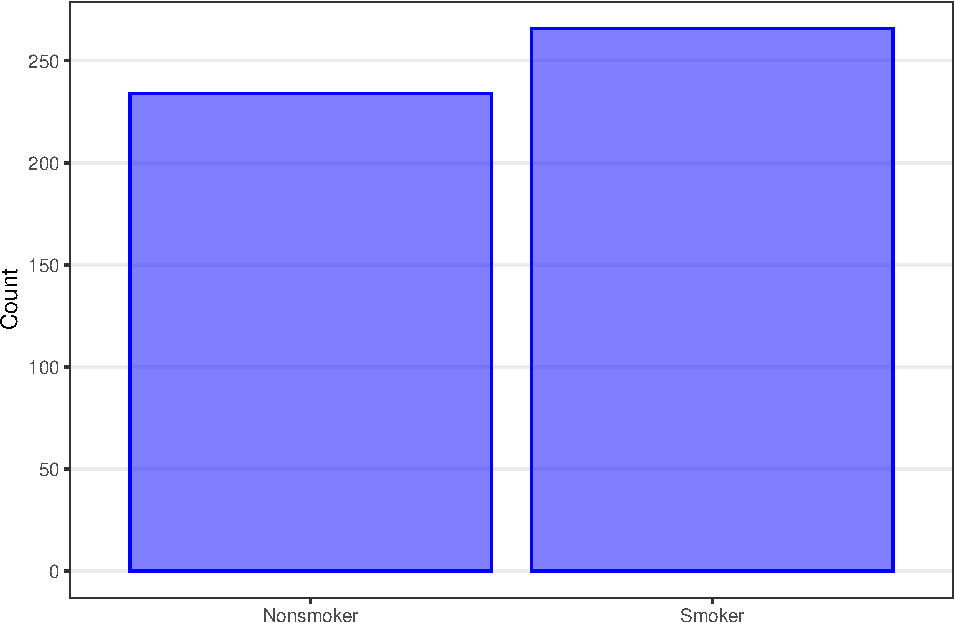
\includegraphics{biostat-book_files/figure-latex/unnamed-chunk-5-1.pdf}

\hypertarget{numerical-data}{%
\subsection{Numerical Data}\label{numerical-data}}

There are many different ways to summarize numerical data. The most common summaries are measures of center (such as means or medians) and measures of spread (such as standard deviations or interquartile ranges). In addition, we typically want to note any extreme or unusual observations in the data.

If we wanted to pick one number to represent a set of data, we'd probably want to pick the value that indicates the center or central tendency of the data values, or the one that is a ``typical'' or average value.

However, we know that there will (most likely) be variability in our data. That is, not all of the values will equal each other. So, the measure of center should not be our only summary measure for numerical data. We are also interested in how spread out, or how varied, our data values are from one another. We do this by computing measures of spread.

There are other summary measures that we may compute as well to understand our data, such as percentiles or the minimum or maximum.

Finally, we want to note if there are any observations that are very different or unusual from all of the other observations in the sample.

\hypertarget{measures-of-center}{%
\subsubsection{Measures of Center}\label{measures-of-center}}

\hypertarget{mean}{%
\paragraph{Mean}\label{mean}}

Some measures of center use the values of the variable. The individual values in the sample are denoted as \(x\) with a subscript \(i\), where \(i\) runs from 1 to the number of observations in our data. For example, the first observation is \(x_1\), the second observation is \(x_2\), and so on. The mean (or average) value, noted as \(\bar{x}\) (pronounced x-bar), is the result of adding up all the individual values, \(x_i\), and then dividing by the number of observations in our sample, denoted by \(n\).

\[
\bar{x} = \frac{\Sigma x_i}{n}
\]
In our Blood Pressure example, when we add up the blood pressure measurements for all 500 adults and divide by 500, we get a mean value of 145 mm Hg.

Note that the mean is calculated using all values in the dataset. If there is one observation or several observations that are much higher or lower than the rest of the data, it will raise or lower the mean more than it would if those observations were similar to the rest of the data.

\hypertarget{median}{%
\paragraph{Median}\label{median}}

Sometimes, it makes more sense to summarize the data by the order as opposed to by the value. Why? Because sometimes there are data points that are so different from the rest that they overly influence the mean. For example, let's say our data points were 1, 2, 3, 4, and 100. If we took the average of these 5 data points, we would get the value 22. But does 22 seem to be typical? Or the center value? It is a lot higher than four of the values and much much lower than the fifth. It doesn't seem to represent any portion of the data very well.

One of the features of numerical data is that you can put it in order from smallest to largest. Let's take advantage of this additional feature of numerical data to create different summaries for the typical value and the spread of the data.

When we order the observations from smallest to largest, there will be a middle value. The \textbf{median} is the value of the middle observation in the dataset. (If there are an even number of observations in the dataset, then the median is the average of the two middle values.) The median is also referred to as the \textbf{50th percentile} because 50\% of the observations are below the median and 50\% are above the median.

For the Blood Pressure dataset, if we order the observations from smallest to largest, the middle observation would be between the 250\(^{th}\) and 251\(^{st}\) observations (because there are an even number, 500, of observations in this dataset). When we average these two values, we get a median of 140.5 mmHg, which is similar, but not the same, as what we calculated for the mean.

Note that the median is calculated using only the middle value or values. If one observation in the data is much higher or lower than the rest of the data, it will be part of the order of the data, but the value itself is not used to find the median. Therefore, observations that are very different (either higher or lower) than most of the data do not affect the value of the median.

\hypertarget{other-measures-of-center}{%
\paragraph{Other Measures of Center}\label{other-measures-of-center}}

Other measures of center that are encountered in the medince and public health include the \textbf{trimmed mean} and the \textbf{geometric mean}.

To calculate a trimmed mean, a specified percentage of the highest and lowest values for that variable are excluded before calculation of the mean. For example, the 10\% trimmed mean would exclude the highest 10\% and lowest 10\% of the observations and then a mean would be calculated based on the included observations (the middle 80\% of the data). This makes the trimmed mean less sensitive to those observations that are much higher or lower than the rest of the data.

To calculate the geometric mean, the data are first log-transformed, then the mean is calculated on the log scale, and lastly, the mean is transformed back to the original scale. The geometric mean can be useful for summarizing highly skewed data.

\hypertarget{literature}{%
\chapter{Literature}\label{literature}}

Here is a review of existing methods.

\hypertarget{methods}{%
\chapter{Methods}\label{methods}}

We describe our methods in this chapter.

\hypertarget{applications}{%
\chapter{Applications}\label{applications}}

Some \emph{significant} applications are demonstrated in this chapter.

\hypertarget{example-one}{%
\section{Example one}\label{example-one}}

\hypertarget{example-two}{%
\section{Example two}\label{example-two}}

\hypertarget{final-words}{%
\chapter{Final Words}\label{final-words}}

We have finished a nice book.

  \bibliography{book.bib,packages.bib}

\end{document}
